% !TEX program = xelatex
% Diccionario de Datos -- Sistema de Inventario + POS (Peterby's)
% Compilar:  latexmk -xelatex -output-directory=../_build diccionario-de-datos.tex
\documentclass[11pt]{article}

\usepackage{fontspec}
\setmainfont{Latin Modern Roman}
\setsansfont{Latin Modern Sans}
\setmonofont{Latin Modern Mono}[Scale=0.92]
\usepackage[spanish,es-tabla,es-nodecimaldot]{babel}
\usepackage{microtype}
\usepackage[a4paper,margin=2.3cm,headheight=22pt]{geometry}
\usepackage{xcolor}
\usepackage{booktabs}
\usepackage{array}
\usepackage{longtable}
\usepackage{graphicx}
\usepackage{enumitem}
\usepackage{titlesec}
\usepackage{fancyhdr}
\usepackage[strings]{underscore}
\usepackage{caption}
\usepackage{hyperref}

\definecolor{brand}{HTML}{34508A}
\definecolor{brandlight}{HTML}{EAF0FA}
\definecolor{rule}{HTML}{C5CEE0}

\hypersetup{colorlinks=true, linkcolor=brand, urlcolor=brand,
  pdftitle={Diccionario de Datos -- Sistema de Inventario Peterby's},
  pdfauthor={Equipo de Ingenieria de Software}}

\captionsetup{font=small, labelfont={bf,color=brand}}

% --- Encabezado / pie ---
\pagestyle{fancy}
\fancyhf{}
\renewcommand{\headrulewidth}{0.6pt}
\renewcommand{\headrule}{\hbox to\headwidth{\color{rule}\leaders\hrule height \headrulewidth\hfill}}
\fancyhead[L]{\small\sffamily\color{brand}Diccionario de Datos}
\fancyhead[R]{\small\sffamily Peterby's POS}
\fancyfoot[C]{\small\sffamily\thepage}

% --- Titulos de seccion ---
\titleformat{\section}{\Large\sffamily\bfseries\color{brand}}{\thesection.}{0.5em}{}
\titleformat{\subsection}{\large\sffamily\bfseries\color{brand!85!black}}{\thesubsection}{0.6em}{}
\titlespacing*{\subsection}{0pt}{1.4ex plus 1ex}{0.6ex}

% --- Entorno: tabla de campos de una entidad ---
% longtable (no tabularx) para poder envolverlo en un entorno propio.
\newenvironment{campos}{%
  \par\footnotesize
  \setlength{\LTpre}{0.3ex}\setlength{\LTpost}{0.6ex}
  \begin{longtable}{@{}>{\ttfamily}p{0.165\linewidth} >{\ttfamily}p{0.150\linewidth} p{0.205\linewidth} >{\raggedright\arraybackslash}p{0.385\linewidth}@{}}
  \toprule
  \normalfont\bfseries Campo & \normalfont\bfseries Tipo & \normalfont\bfseries Restricciones & \normalfont\bfseries Descripción \\
  \midrule \endfirsthead
  \multicolumn{4}{@{}l}{\footnotesize\itshape \dots\ continuación}\\[0.3ex]
  \toprule
  \normalfont\bfseries Campo & \normalfont\bfseries Tipo & \normalfont\bfseries Restricciones & \normalfont\bfseries Descripción \\
  \midrule \endhead
  \midrule \multicolumn{4}{r@{}}{\footnotesize\itshape continúa en la siguiente página}\\ \endfoot
  \bottomrule \endlastfoot
}{%
  \end{longtable}\par
}

% Proposito de una tabla
\newcommand{\proposito}[1]{\par\vspace{0.2ex}\noindent\colorbox{brandlight}{\parbox{\dimexpr\linewidth-2\fboxsep}{\small\textbf{Propósito.} #1}}\par\vspace{0.8ex}}

% Atajos para restricciones (evitan caracteres conflictivos)
\newcommand{\pk}{\textsc{pk}}
\newcommand{\fk}[1]{\textsc{fk}: \texttt{#1}}
\newcommand{\nn}{\textsc{not null}}
\newcommand{\uq}{\textsc{unique}}

\begin{document}

% ===================== PORTADA =====================
\begin{titlepage}
\centering
\vspace*{1.2cm}
{\sffamily\large Instituto Politécnico Nacional}\\[0.2cm]
{\sffamily Escuela Superior de Cómputo --- ESCOM}\\[0.2cm]
{\sffamily Ingeniería de Software}\\[2.2cm]

{\color{rule}\rule{\linewidth}{0.8pt}}\\[0.6cm]
{\Huge\sffamily\bfseries\color{brand} Diccionario de Datos}\\[0.5cm]
{\large\sffamily Sistema de Inventario con Punto de Venta\\ y Análisis Predictivo de Reabastecimiento}\\[0.3cm]
{\large\sffamily\itshape Tienda de ropa Peterby's}\\[0.4cm]
{\color{rule}\rule{\linewidth}{0.8pt}}\\[1.6cm]

\begin{tabular}{rl}
\sffamily\bfseries Motor de base de datos: & \sffamily SQLite 3 \\[0.2cm]
\sffamily\bfseries Tablas documentadas: & \sffamily 24 \\[0.2cm]
\sffamily\bfseries Documento: & \sffamily Análisis y diseño de datos \\
\end{tabular}

\vfill
{\sffamily\small Diciembre 2025}
\end{titlepage}

% ===================== INDICE =====================
\tableofcontents
\clearpage

% ===================== 1. INTRODUCCION =====================
\section{Introducción}

Este documento describe la estructura de la base de datos del sistema de
inventario y punto de venta (POS) de la tienda Peterby's. Para cada una de las
24 tablas se indica su \textbf{propósito} y, por cada campo, su \textbf{tipo},
\textbf{restricciones} y una \textbf{descripción} funcional. La fuente de diseño
es el modelo entidad-relación de la Figura~\ref{fig:der}; el archivo
\texttt{database/schema.sql} es su traducción 1:1 al lenguaje de definición de
datos (DDL) de SQLite.

\subsection*{Convenciones de lectura}
\begin{itemize}[leftmargin=1.4em, itemsep=0.2ex]
  \item Los nombres de tablas y campos están en español sin acentos (ASCII),
        para coincidir con el código del sistema.
  \item Toda tabla tiene clave primaria \texttt{id} de tipo \texttt{INTEGER}
        autoincremental (\pk).
  \item Las claves foráneas usan el sufijo \texttt{\_id} y se anotan como
        \fk{tabla\_referenciada}.
  \item \nn{} = obligatorio; \uq{} = valor único; \textsc{def} = valor por
        defecto; \textsc{check} = valor controlado o regla a nivel de datos.
  \item SQLite no impone la longitud de \texttt{VARCHAR} ni la escala de
        \texttt{NUMERIC} (son afinidad de tipo); se conservan como documentación
        del dominio. Las restricciones efectivamente impuestas son \nn,
        \uq, \textsc{foreign key} y \textsc{check}.
\end{itemize}

\subsection*{Organización de las tablas}
Las tablas se agrupan en cinco bloques temáticos:
\begin{enumerate}[label=\textbf{\Alph*.}, leftmargin=1.8em, itemsep=0.2ex]
  \item \textbf{Catálogos base} --- colores, marcas, tallas, temporadas,
        categorías, proveedores, clientes y usuarios.
  \item \textbf{Productos y surtido} --- productos, variantes, imágenes,
        relación con proveedores y outfits.
  \item \textbf{Operación comercial} --- ventas, detalle de ventas, pagos,
        movimientos de inventario y devoluciones.
  \item \textbf{Promociones} --- promociones y su relación con variantes.
  \item \textbf{Inteligencia del sistema} --- alertas, bitácora de auditoría y
        predicciones de reabastecimiento.
\end{enumerate}

\begin{figure}[htbp]
  \centering
  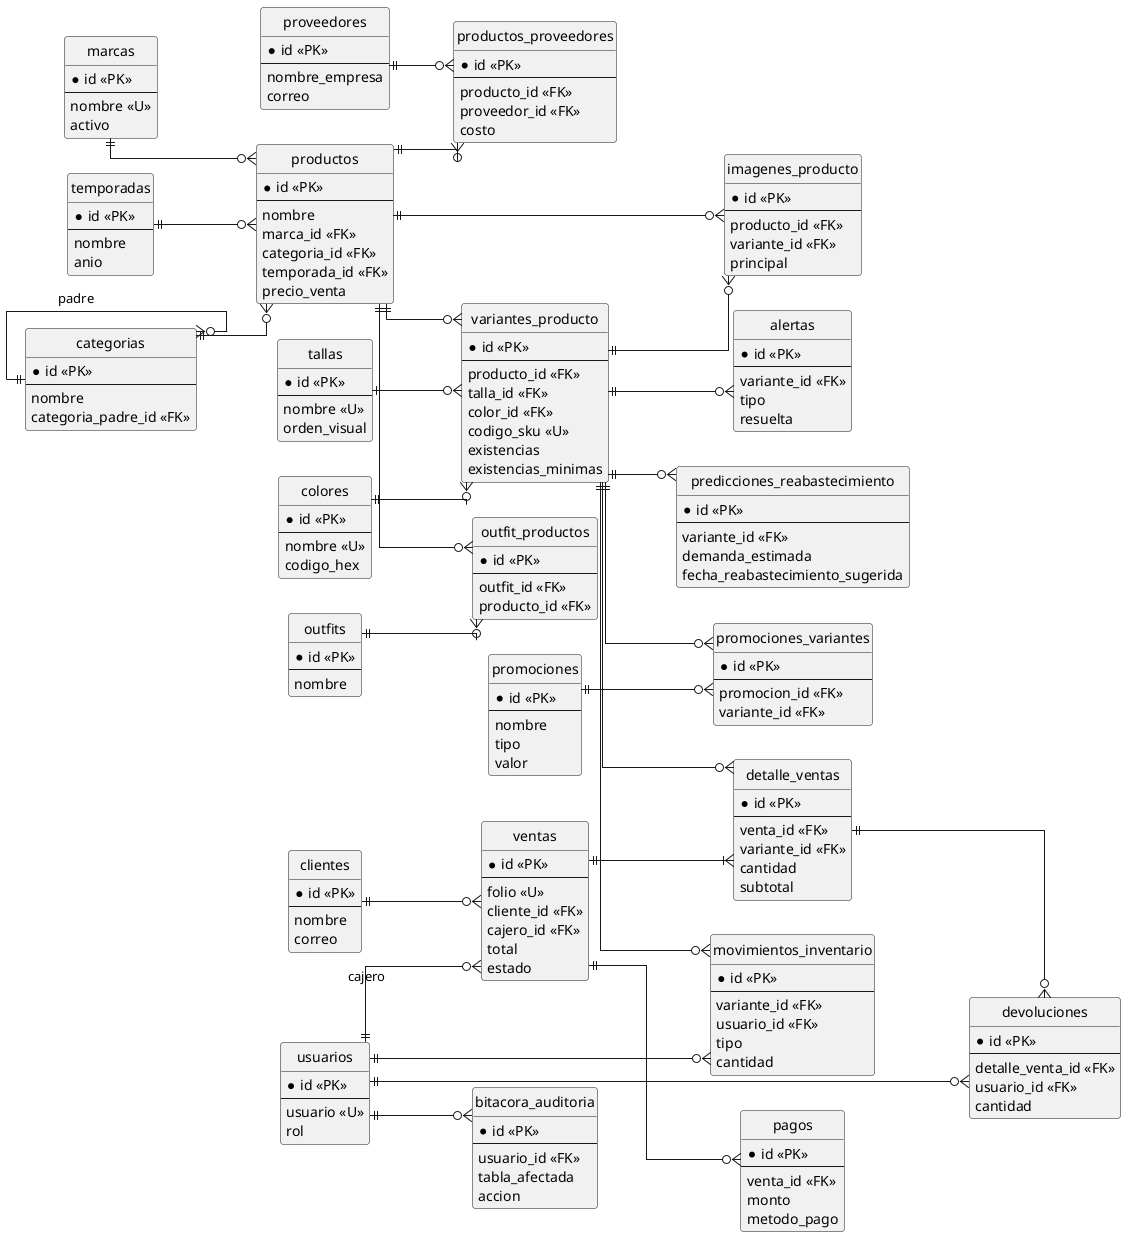
\includegraphics[width=\linewidth,height=0.82\textheight,keepaspectratio]{diagramas/der.png}
  \caption{Modelo entidad-relación (DER) del sistema. Notación de pie de cuervo.}
  \label{fig:der}
\end{figure}
\clearpage

% ===================== 2. CATALOGOS BASE =====================
\section{Catálogos base}

\subsection{colores}
\proposito{Paleta de colores disponible para las variantes de producto.}
\begin{campos}
id          & INTEGER       & \pk{}                       & Identificador del color. \\
nombre      & VARCHAR(50)   & \nn, \uq                    & Nombre del color (p. ej. Negro, Azul marino). \\
codigo\_hex & VARCHAR(7)    & \textsc{def} '\#000000', \textsc{check} formato \#RRGGBB & Código hexadecimal para mostrar el color en la interfaz. \\
\end{campos}

\subsection{marcas}
\proposito{Marcas o etiquetas comerciales bajo las que se clasifican los productos.}
\begin{campos}
id             & INTEGER    & \pk{}                & Identificador de la marca. \\
nombre         & VARCHAR(100) & \nn, \uq           & Nombre de la marca. \\
descripcion    & TEXT       &                      & Descripción libre de la marca. \\
url\_logo      & TEXT       &                      & Ruta o URL del logotipo. \\
activo         & INTEGER    & \nn, \textsc{def} 1, \textsc{check} 0/1 & Marca habilitada (1) o deshabilitada (0). \\
fecha\_creacion & TIMESTAMP & \textsc{def} ahora   & Fecha y hora de alta del registro. \\
\end{campos}

\subsection{tallas}
\proposito{Catálogo de tallas; \texttt{orden\_visual} fija el orden en que se muestran.}
\begin{campos}
id            & INTEGER     & \pk{}              & Identificador de la talla. \\
nombre        & VARCHAR(20) & \nn, \uq           & Etiqueta de talla (XS, S, M, L, 28, 30\dots). \\
descripcion   & TEXT        &                    & Descripción o equivalencia de la talla. \\
orden\_visual & INTEGER     & \nn, \textsc{def} 0 & Posición para ordenar las tallas en la interfaz. \\
\end{campos}

\subsection{temporadas}
\proposito{Temporadas comerciales (p. ej. Primavera-Verano 2025) para clasificar el surtido.}
\begin{campos}
id            & INTEGER      & \pk{}             & Identificador de la temporada. \\
nombre        & VARCHAR(100) & \nn               & Nombre de la temporada. \\
anio          & INTEGER      & \nn, \textsc{check} 2000--2100 & Año al que corresponde. \\
activo        & INTEGER      & \nn, \textsc{def} 1, \textsc{check} 0/1 & Temporada vigente. \\
fecha\_inicio & DATE         &                   & Inicio de la temporada. \\
fecha\_fin    & DATE         & \textsc{check} $\geq$ inicio & Fin de la temporada (no anterior al inicio). \\
\end{campos}

\subsection{categorias}
\proposito{Categorías de producto, jerárquicas mediante autorreferencia (\texttt{categoria\_padre\_id}).}
\begin{campos}
id                  & INTEGER      & \pk{}        & Identificador de la categoría. \\
nombre              & VARCHAR(100) & \nn          & Nombre de la categoría. \\
descripcion         & TEXT         &              & Descripción. \\
categoria\_padre\_id & INTEGER     & \fk{categorias}, \textsc{on del} set null & Categoría padre; nulo si es categoría raíz. \\
activo              & INTEGER      & \nn, \textsc{def} 1, \textsc{check} 0/1 & Categoría habilitada. \\
\end{campos}

\subsection{proveedores}
\proposito{Proveedores mayoristas que surten la mercancía de la tienda.}
\begin{campos}
id              & INTEGER      & \pk{}      & Identificador del proveedor. \\
nombre\_empresa & VARCHAR(200) & \nn        & Razón social del proveedor. \\
nombre\_contacto & VARCHAR(200) &           & Persona de contacto. \\
telefono        & VARCHAR(30)  &            & Teléfono. \\
correo          & VARCHAR(150) &            & Correo electrónico (campo ampliado; antes 25). \\
pais            & VARCHAR(100) &            & País. \\
ciudad          & VARCHAR(100) &            & Ciudad. \\
direccion       & TEXT         &            & Dirección. \\
tipos\_producto & VARCHAR(200) &            & Tipos de mercancía que surte. \\
activo          & INTEGER      & \nn, \textsc{def} 1, \textsc{check} 0/1 & Proveedor activo. \\
fecha\_creacion & TIMESTAMP    & \textsc{def} ahora & Alta del registro. \\
\end{campos}

\subsection{clientes}
\proposito{Clientes de la tienda; opcionales en cada venta y base para el análisis de ventas.}
\begin{campos}
id             & INTEGER      & \pk{}      & Identificador del cliente. \\
nombre         & VARCHAR(100) & \nn        & Nombre(s). \\
apellido       & VARCHAR(100) &            & Apellidos. \\
telefono       & VARCHAR(20)  &            & Teléfono. \\
correo         & VARCHAR(100) &            & Correo electrónico. \\
direccion      & TEXT         &            & Dirección. \\
ciudad         & VARCHAR(100) &            & Ciudad. \\
estado         & VARCHAR(100) &            & Entidad federativa (no confundir con estatus). \\
codigo\_postal & VARCHAR(10)  &            & Código postal. \\
nacimiento     & DATE         &            & Fecha de nacimiento. \\
genero         & VARCHAR(20)  & \textsc{check} Masculino, Femenino, Otro (o nulo) & Género del cliente. \\
fecha\_creacion & TIMESTAMP   & \textsc{def} ahora & Alta del registro. \\
\end{campos}

\subsection{usuarios}
\proposito{Operadores del sistema. El campo \texttt{rol} determina los permisos (ver casos de uso).}
\begin{campos}
id              & INTEGER     & \pk{}     & Identificador del usuario. \\
usuario         & VARCHAR(50) & \nn, \uq  & Nombre de usuario para iniciar sesión. \\
nombre\_completo & VARCHAR(100) &          & Nombre completo. \\
correo          & VARCHAR(100) &           & Correo electrónico. \\
hash\_contrasena & TEXT        & \nn       & Hash de la contraseña (nunca se guarda en claro). \\
rol             & VARCHAR(25) & \nn, \textsc{def} 'Vendedor', \textsc{check} Gerente, Vendedor & Rol que determina los permisos. \\
activo          & INTEGER     & \nn, \textsc{def} 1, \textsc{check} 0/1 & Cuenta habilitada. \\
datos\_perfil   & TEXT        &           & JSON opcional con preferencias del usuario. \\
fecha\_creacion & TIMESTAMP   & \textsc{def} ahora & Alta de la cuenta. \\
ultimo\_acceso  & TIMESTAMP   &           & Fecha del último inicio de sesión. \\
\end{campos}

% ===================== 3. PRODUCTOS Y SURTIDO =====================
\section{Productos y surtido}

\subsection{productos}
\proposito{Producto ``padre'' (modelo). El stock real reside en \texttt{variantes\_producto}.}
\begin{campos}
id                  & INTEGER       & \pk{}    & Identificador del producto. \\
nombre              & VARCHAR(200)  & \nn      & Nombre del producto (modelo). \\
descripcion         & TEXT          &          & Descripción. \\
marca\_id           & INTEGER       & \fk{marcas}, \textsc{on del} set null & Marca. \\
categoria\_id       & INTEGER       & \fk{categorias}, \textsc{on del} set null & Categoría. \\
temporada\_id       & INTEGER       & \fk{temporadas}, \textsc{on del} set null & Temporada. \\
genero              & VARCHAR(50)   &          & Público objetivo (Hombre / Mujer / Unisex). \\
costo\_base         & NUMERIC(12,2) & \nn, \textsc{def} 0, \textsc{check} $\geq 0$ & Costo de referencia del producto. \\
precio\_venta       & NUMERIC(12,2) & \nn, \textsc{def} 0, \textsc{check} $\geq 0$ & Precio sugerido (la variante puede sobreescribirlo). \\
color\_venta        & VARCHAR(100)  &          & Color principal mostrado. \\
activo              & INTEGER       & \nn, \textsc{def} 1, \textsc{check} 0/1 & Producto a la venta. \\
fecha\_creacion     & TIMESTAMP     & \textsc{def} ahora & Alta. \\
fecha\_actualizacion & TIMESTAMP    & \textsc{def} ahora & Última modificación. \\
\end{campos}

\subsection{variantes\_producto}
\proposito{Combinación vendible (producto + talla + color). Es la unidad real de inventario.}
\begin{campos}
id                   & INTEGER       & \pk{}   & Identificador de la variante. \\
producto\_id         & INTEGER       & \nn, \fk{productos}, \textsc{on del} cascade & Producto padre. \\
talla\_id            & INTEGER       & \fk{tallas}, \textsc{on del} set null & Talla. \\
color\_id            & INTEGER       & \fk{colores}, \textsc{on del} set null & Color. \\
codigo\_sku          & VARCHAR(100)  & \uq     & SKU interno. \\
codigo\_barras       & VARCHAR(100)  & \uq     & Código de barras. \\
existencias          & INTEGER       & \nn, \textsc{def} 0, \textsc{check} $\geq 0$ & Stock actual; nunca negativo (RN-008). \\
existencias\_minimas & INTEGER       & \nn, \textsc{def} 5, \textsc{check} $\geq 0$ & Stock mínimo; dispara alertas (RN-003). \\
precio\_venta        & NUMERIC(12,2) & \textsc{check} $\geq 0$ o nulo & Precio específico de la variante. \\
peso                 & NUMERIC(10,3) &         & Peso en kilogramos (antes sin escala). \\
activo               & INTEGER       & \nn, \textsc{def} 1, \textsc{check} 0/1 & Variante a la venta. \\
fecha\_creacion      & TIMESTAMP     & \textsc{def} ahora & Alta. \\
fecha\_actualizacion & TIMESTAMP     & \textsc{def} ahora & Última modificación. \\
\end{campos}

\subsection{imagenes\_producto}
\proposito{Imágenes asociadas a un producto o a una variante concreta.}
\begin{campos}
id          & INTEGER & \pk{}       & Identificador de la imagen. \\
producto\_id & INTEGER & \fk{productos}, \textsc{on del} cascade & Producto asociado (opcional). \\
variante\_id & INTEGER & \fk{variantes\_producto}, \textsc{on del} cascade & Variante asociada (opcional). \\
url\_imagen & TEXT    & \nn         & Ruta o URL de la imagen. \\
principal   & INTEGER & \nn, \textsc{def} 0, \textsc{check} 0/1 & Imagen principal del producto/variante. \\
orden       & INTEGER & \nn, \textsc{def} 0 & Orden de despliegue. \\
\multicolumn{4}{@{}p{0.97\linewidth}}{\footnotesize\itshape Regla de tabla: \textsc{check} \texttt{producto\_id} o \texttt{variante\_id} no nulo (al menos uno).} \\
\end{campos}

\subsection{productos\_proveedores}
\proposito{Relación N:M entre productos y proveedores con su costo y plazo de entrega.}
\begin{campos}
id                  & INTEGER       & \pk{}   & Identificador del registro. \\
producto\_id        & INTEGER       & \nn, \fk{productos}, \textsc{on del} cascade & Producto. \\
proveedor\_id       & INTEGER       & \nn, \fk{proveedores}, \textsc{on del} cascade & Proveedor. \\
costo               & NUMERIC(12,2) & \textsc{check} $\geq 0$ & Costo de compra a ese proveedor. \\
tiempo\_entrega\_dias & INTEGER     & \textsc{check} $\geq 0$ & Días estimados de entrega. \\
\multicolumn{4}{@{}p{0.97\linewidth}}{\footnotesize\itshape Regla de tabla: \uq{} (\texttt{producto\_id}, \texttt{proveedor\_id}).} \\
\end{campos}

\subsection{outfits}
\proposito{Conjuntos sugeridos de prendas (venta cruzada / cross-selling).}
\begin{campos}
id          & INTEGER      & \pk{}   & Identificador del outfit. \\
nombre      & VARCHAR(200) &         & Nombre del conjunto. \\
descripcion & TEXT         &         & Descripción. \\
url\_imagen & TEXT         &         & Imagen del outfit. \\
activo      & INTEGER      & \nn, \textsc{def} 1, \textsc{check} 0/1 & Outfit visible. \\
\end{campos}

\subsection{outfit\_productos}
\proposito{Productos que componen cada outfit (relación N:M).}
\begin{campos}
id          & INTEGER & \pk{}    & Identificador del registro. \\
outfit\_id  & INTEGER & \nn, \fk{outfits}, \textsc{on del} cascade & Outfit. \\
producto\_id & INTEGER & \nn, \fk{productos}, \textsc{on del} cascade & Producto integrante. \\
\multicolumn{4}{@{}p{0.97\linewidth}}{\footnotesize\itshape Regla de tabla: \uq{} (\texttt{outfit\_id}, \texttt{producto\_id}).} \\
\end{campos}

% ===================== 4. OPERACION COMERCIAL =====================
\section{Operación comercial}

\subsection{ventas}
\proposito{Encabezado de cada ticket de venta.}
\begin{campos}
id          & INTEGER       & \pk{}     & Identificador de la venta. \\
folio       & VARCHAR(50)   & \uq       & Folio del ticket. \\
cliente\_id & INTEGER       & \fk{clientes}, \textsc{on del} set null & Cliente (opcional). \\
cajero\_id  & INTEGER       & \fk{usuarios}, \textsc{on del} set null & Usuario que realiza el cobro. \\
subtotal    & NUMERIC(12,2) & \nn, \textsc{def} 0, \textsc{check} $\geq 0$ & Suma de partidas antes de impuestos y descuentos. \\
descuentos  & NUMERIC(12,2) & \nn, \textsc{def} 0, \textsc{check} $\geq 0$ & Descuentos aplicados al total. \\
impuestos   & NUMERIC(12,2) & \nn, \textsc{def} 0, \textsc{check} $\geq 0$ & Impuestos. \\
total       & NUMERIC(12,2) & \nn, \textsc{def} 0, \textsc{check} $\geq 0$ & Total a pagar. \\
metodo\_pago & VARCHAR(50)  & \textsc{check} Efectivo, Tarjeta, Mixto (o nulo) & Método de pago global del ticket. \\
estado      & VARCHAR(30)   & \nn, \textsc{def} 'completada', \textsc{check} completada, cancelada, devuelta & Estado de la venta. \\
notas       & TEXT          &           & Observaciones (campo ampliado; antes 50). \\
fecha\_venta & TIMESTAMP    & \textsc{def} ahora & Fecha y hora de la venta. \\
\end{campos}

\subsection{detalle\_ventas}
\proposito{Renglones (partidas) de cada venta, a nivel de variante.}
\begin{campos}
id              & INTEGER       & \pk{}   & Identificador del renglón. \\
venta\_id       & INTEGER       & \nn, \fk{ventas}, \textsc{on del} cascade & Venta a la que pertenece. \\
variante\_id    & INTEGER       & \nn, \fk{variantes\_producto}, \textsc{on del} restrict & Variante vendida (no se borra si tiene ventas). \\
cantidad        & INTEGER       & \nn, \textsc{def} 1, \textsc{check} $>0$ & Unidades vendidas. \\
precio\_unitario & NUMERIC(12,2) & \nn, \textsc{check} $\geq 0$ & Precio unitario aplicado. \\
descuentos\_item & NUMERIC(12,2) & \nn, \textsc{def} 0, \textsc{check} $\geq 0$ & Descuento del renglón. \\
subtotal        & NUMERIC(12,2) & \nn, \textsc{check} $\geq 0$ & Importe del renglón. \\
\end{campos}

\subsection{pagos}
\proposito{Pagos aplicados a una venta; varios renglones permiten el pago mixto.}
\begin{campos}
id          & INTEGER       & \pk{}   & Identificador del pago. \\
venta\_id   & INTEGER       & \nn, \fk{ventas}, \textsc{on del} cascade & Venta pagada. \\
monto       & NUMERIC(12,2) & \nn, \textsc{check} $>0$ & Importe de este pago. \\
metodo\_pago & VARCHAR(50)  & \nn, \textsc{check} Efectivo, Tarjeta, Transferencia & Método de este pago (la combinación produce ``Mixto''). \\
referencia  & VARCHAR(100)  &         & Autorización o folio externo. \\
fecha\_pago & TIMESTAMP     & \textsc{def} ahora & Fecha del pago. \\
\end{campos}

\subsection{movimientos\_inventario}
\proposito{Kardex: registra toda entrada/salida de existencias por variante (trazabilidad).}
\begin{campos}
id                  & INTEGER     & \pk{}   & Identificador del movimiento. \\
variante\_id        & INTEGER     & \nn, \fk{variantes\_producto}, \textsc{on del} cascade & Variante afectada. \\
tipo                & VARCHAR(50) & \nn, \textsc{check} venta, compra, ajuste, devolucion & Tipo de movimiento. \\
cantidad            & INTEGER     & \nn, \textsc{check} $\neq 0$ & Unidades ($+$ entra, $-$ sale). \\
existencias\_antes  & INTEGER     & \nn, \textsc{check} $\geq 0$ & Stock previo al movimiento. \\
existencias\_despues & INTEGER    & \nn, \textsc{check} $\geq 0$ & Stock resultante. \\
referencia          & TEXT        &         & Folio de venta o compra que origina el movimiento. \\
usuario\_id         & INTEGER     & \fk{usuarios}, \textsc{on del} set null & Usuario responsable. \\
fecha               & TIMESTAMP   & \textsc{def} ahora & Fecha del movimiento. \\
\end{campos}

\subsection{devoluciones}
\proposito{Devolución de un renglón de venta; reintegra stock al inventario.}
\begin{campos}
id                & INTEGER   & \pk{}   & Identificador de la devolución. \\
detalle\_venta\_id & INTEGER  & \nn, \fk{detalle\_ventas}, \textsc{on del} restrict & Renglón de venta devuelto. \\
usuario\_id       & INTEGER   & \fk{usuarios}, \textsc{on del} set null & Usuario que procesa la devolución. \\
cantidad          & INTEGER   & \nn, \textsc{check} $>0$ & Unidades devueltas. \\
motivo            & TEXT      &         & Motivo de la devolución. \\
fecha             & TIMESTAMP & \textsc{def} ahora & Fecha de la devolución. \\
\end{campos}

% ===================== 5. PROMOCIONES =====================
\section{Promociones}

\subsection{promociones}
\proposito{Promociones con vigencia: descuento por porcentaje o por monto fijo.}
\begin{campos}
id           & INTEGER       & \pk{}   & Identificador de la promoción. \\
nombre       & VARCHAR(200)  & \nn     & Nombre de la promoción. \\
tipo         & VARCHAR(50)   & \nn, \textsc{check} porcentaje, monto\_fijo & Tipo de descuento. \\
valor        & NUMERIC(12,2) & \nn, \textsc{check} $\geq 0$ & Porcentaje o monto (tope se valida en la app, RN-011). \\
fecha\_inicio & DATE         &         & Inicio de vigencia. \\
fecha\_fin   & DATE          & \textsc{check} $\geq$ inicio & Fin de vigencia (RN-004). \\
activo       & INTEGER       & \nn, \textsc{def} 1, \textsc{check} 0/1 & Promoción vigente. \\
\end{campos}

\subsection{promociones\_variantes}
\proposito{Variantes alcanzadas por cada promoción (relación N:M).}
\begin{campos}
id           & INTEGER & \pk{}   & Identificador del registro. \\
promocion\_id & INTEGER & \nn, \fk{promociones}, \textsc{on del} cascade & Promoción. \\
variante\_id & INTEGER & \nn, \fk{variantes\_producto}, \textsc{on del} cascade & Variante alcanzada. \\
\multicolumn{4}{@{}p{0.97\linewidth}}{\footnotesize\itshape Regla de tabla: \uq{} (\texttt{promocion\_id}, \texttt{variante\_id}).} \\
\end{campos}

% ===================== 6. INTELIGENCIA DEL SISTEMA =====================
\section{Inteligencia del sistema}

\subsection{alertas}
\proposito{Alertas automáticas de stock o reabastecimiento que se muestran al usuario.}
\begin{campos}
id             & INTEGER      & \pk{}   & Identificador de la alerta. \\
variante\_id   & INTEGER      & \fk{variantes\_producto}, \textsc{on del} cascade & Variante relacionada. \\
tipo           & VARCHAR(100) & \nn, \textsc{check} stock\_minimo, stock\_agotado, reabastecimiento & Tipo de alerta. \\
mensaje        & TEXT         &         & Texto descriptivo de la alerta. \\
resuelta       & INTEGER      & \nn, \textsc{def} 0, \textsc{check} 0/1 & Atendida (1) o pendiente (0). \\
fecha\_creacion & TIMESTAMP   & \textsc{def} ahora & Fecha de generación. \\
\end{campos}

\subsection{bitacora\_auditoria}
\proposito{Registro de cambios sensibles: quién, en qué tabla, qué acción y los valores antes/después.}
\begin{campos}
id                & INTEGER      & \pk{}   & Identificador del asiento. \\
usuario\_id       & INTEGER      & \fk{usuarios}, \textsc{on del} set null & Usuario que ejecutó la acción. \\
tabla\_afectada   & VARCHAR(100) & \nn     & Tabla modificada. \\
accion            & VARCHAR(30)  & \nn, \textsc{check} INSERT, UPDATE, DELETE & Operación realizada. \\
detalles\_anterior & TEXT        &         & Snapshot JSON del estado previo. \\
detalles\_nuevo   & TEXT         &         & Snapshot JSON del estado nuevo. \\
fecha             & TIMESTAMP    & \textsc{def} ahora & Fecha del cambio. \\
\end{campos}

\subsection{predicciones\_reabastecimiento}
\proposito{Salida del modelo Random Forest: demanda estimada y fecha sugerida de reabastecimiento por variante.}
\begin{campos}
id                              & INTEGER       & \pk{}   & Identificador de la predicción. \\
variante\_id                    & INTEGER       & \nn, \fk{variantes\_producto}, \textsc{on del} cascade & Variante evaluada. \\
demanda\_estimada               & NUMERIC(12,2) & \textsc{check} $\geq 0$ & Demanda estimada por el modelo. \\
dias\_estimados                 & INTEGER       & \textsc{check} $\geq 0$ & Días estimados de cobertura del stock. \\
nivel\_confianza                & NUMERIC(5,2)  & \textsc{check} 0--100 & Confianza de la predicción (porcentaje). \\
fecha\_prediccion               & TIMESTAMP     & \textsc{def} ahora & Cuándo se generó la predicción. \\
fecha\_reabastecimiento\_sugerida & DATE        &         & Fecha sugerida para reabastecer. \\
modelo\_id                      & VARCHAR(100)  &         & Identificador o versión del modelo. \\
detalles                        & TEXT          &         & JSON con variables de entrada y métricas. \\
\end{campos}

% ===================== ANEXOS =====================
\section{Anexos}

\subsection{Catálogos de valores controlados}
La siguiente tabla resume los campos cuyo valor está restringido por una
cláusula \textsc{check} a un conjunto cerrado de valores.

\begin{center}\footnotesize
\setlength{\LTpre}{0.3ex}
\begin{longtable}{@{}>{\ttfamily}p{0.27\linewidth} >{\raggedright\arraybackslash}p{0.66\linewidth}@{}}
\toprule
\normalfont\bfseries Tabla.campo & \normalfont\bfseries Valores permitidos \\ \midrule \endhead
usuarios.rol                 & Gerente, Vendedor \\
ventas.estado                & completada, cancelada, devuelta \\
ventas.metodo\_pago          & Efectivo, Tarjeta, Mixto \\
pagos.metodo\_pago           & Efectivo, Tarjeta, Transferencia \\
movimientos\_inventario.tipo & venta, compra, ajuste, devolucion \\
promociones.tipo             & porcentaje, monto\_fijo \\
alertas.tipo                 & stock\_minimo, stock\_agotado, reabastecimiento \\
bitacora\_auditoria.accion   & INSERT, UPDATE, DELETE \\
clientes.genero              & Masculino, Femenino, Otro (o nulo) \\
\bottomrule
\end{longtable}
\end{center}

\subsection{Notas de alineación con el prototipo}
\begin{itemize}[leftmargin=1.4em, itemsep=0.4ex]
  \item \textbf{Roles de usuario.} El análisis (factibilidad operativa) define
        dos roles operativos: \textbf{Gerente} y \textbf{Vendedor}; este
        diccionario alinea \texttt{usuarios.rol} a ese par. El prototipo actual
        emplea los nombres \texttt{Admin}/\texttt{Empleado}/\texttt{Gerente}
        (con una migración \texttt{Administrador} a \texttt{Admin} y
        \texttt{Cajero} a \texttt{Empleado}). Mapeo recomendado al regenerar la
        base: \texttt{Admin} y \texttt{Gerente} pasan a \texttt{Gerente};
        \texttt{Empleado} y \texttt{Cajero} pasan a \texttt{Vendedor}. Ajustar
        en consecuencia la creación del usuario por defecto.
  \item \textbf{Tipos en SQLite.} \texttt{VARCHAR(n)} y \texttt{NUMERIC(p,s)} se
        conservan como documentación; SQLite no impone longitud ni escala. Las
        garantías reales provienen de \nn, \uq, \textsc{foreign key} y
        \textsc{check}.
  \item \textbf{Reglas de negocio a nivel de datos.} Se aplican mediante
        \textsc{check}: stock no negativo (RN-008), cantidades positivas, precios
        y montos no negativos, y vigencias coherentes (fin $\geq$ inicio). Las
        reglas que cruzan tablas o requieren contexto (p. ej. precio de venta
        mayor al costo, RN-002; tope de promoción, RN-011) se validan en la capa
        de aplicación.
\end{itemize}

\end{document}
